% Options for packages loaded elsewhere
\PassOptionsToPackage{unicode}{hyperref}
\PassOptionsToPackage{hyphens}{url}
%
\documentclass[
]{article}
\usepackage{amsmath,amssymb}
\usepackage{lmodern}
\usepackage{ifxetex,ifluatex}
\ifnum 0\ifxetex 1\fi\ifluatex 1\fi=0 % if pdftex
  \usepackage[T1]{fontenc}
  \usepackage[utf8]{inputenc}
  \usepackage{textcomp} % provide euro and other symbols
\else % if luatex or xetex
  \usepackage{unicode-math}
  \defaultfontfeatures{Scale=MatchLowercase}
  \defaultfontfeatures[\rmfamily]{Ligatures=TeX,Scale=1}
\fi
% Use upquote if available, for straight quotes in verbatim environments
\IfFileExists{upquote.sty}{\usepackage{upquote}}{}
\IfFileExists{microtype.sty}{% use microtype if available
  \usepackage[]{microtype}
  \UseMicrotypeSet[protrusion]{basicmath} % disable protrusion for tt fonts
}{}
\makeatletter
\@ifundefined{KOMAClassName}{% if non-KOMA class
  \IfFileExists{parskip.sty}{%
    \usepackage{parskip}
  }{% else
    \setlength{\parindent}{0pt}
    \setlength{\parskip}{6pt plus 2pt minus 1pt}}
}{% if KOMA class
  \KOMAoptions{parskip=half}}
\makeatother
\usepackage{xcolor}
\IfFileExists{xurl.sty}{\usepackage{xurl}}{} % add URL line breaks if available
\IfFileExists{bookmark.sty}{\usepackage{bookmark}}{\usepackage{hyperref}}
\hypersetup{
  pdftitle={Project 2: Breast Cancer Diagnosis},
  pdfauthor={Xinran Sun},
  hidelinks,
  pdfcreator={LaTeX via pandoc}}
\urlstyle{same} % disable monospaced font for URLs
\usepackage[margin=1in]{geometry}
\usepackage{color}
\usepackage{fancyvrb}
\newcommand{\VerbBar}{|}
\newcommand{\VERB}{\Verb[commandchars=\\\{\}]}
\DefineVerbatimEnvironment{Highlighting}{Verbatim}{commandchars=\\\{\}}
% Add ',fontsize=\small' for more characters per line
\usepackage{framed}
\definecolor{shadecolor}{RGB}{248,248,248}
\newenvironment{Shaded}{\begin{snugshade}}{\end{snugshade}}
\newcommand{\AlertTok}[1]{\textcolor[rgb]{0.94,0.16,0.16}{#1}}
\newcommand{\AnnotationTok}[1]{\textcolor[rgb]{0.56,0.35,0.01}{\textbf{\textit{#1}}}}
\newcommand{\AttributeTok}[1]{\textcolor[rgb]{0.77,0.63,0.00}{#1}}
\newcommand{\BaseNTok}[1]{\textcolor[rgb]{0.00,0.00,0.81}{#1}}
\newcommand{\BuiltInTok}[1]{#1}
\newcommand{\CharTok}[1]{\textcolor[rgb]{0.31,0.60,0.02}{#1}}
\newcommand{\CommentTok}[1]{\textcolor[rgb]{0.56,0.35,0.01}{\textit{#1}}}
\newcommand{\CommentVarTok}[1]{\textcolor[rgb]{0.56,0.35,0.01}{\textbf{\textit{#1}}}}
\newcommand{\ConstantTok}[1]{\textcolor[rgb]{0.00,0.00,0.00}{#1}}
\newcommand{\ControlFlowTok}[1]{\textcolor[rgb]{0.13,0.29,0.53}{\textbf{#1}}}
\newcommand{\DataTypeTok}[1]{\textcolor[rgb]{0.13,0.29,0.53}{#1}}
\newcommand{\DecValTok}[1]{\textcolor[rgb]{0.00,0.00,0.81}{#1}}
\newcommand{\DocumentationTok}[1]{\textcolor[rgb]{0.56,0.35,0.01}{\textbf{\textit{#1}}}}
\newcommand{\ErrorTok}[1]{\textcolor[rgb]{0.64,0.00,0.00}{\textbf{#1}}}
\newcommand{\ExtensionTok}[1]{#1}
\newcommand{\FloatTok}[1]{\textcolor[rgb]{0.00,0.00,0.81}{#1}}
\newcommand{\FunctionTok}[1]{\textcolor[rgb]{0.00,0.00,0.00}{#1}}
\newcommand{\ImportTok}[1]{#1}
\newcommand{\InformationTok}[1]{\textcolor[rgb]{0.56,0.35,0.01}{\textbf{\textit{#1}}}}
\newcommand{\KeywordTok}[1]{\textcolor[rgb]{0.13,0.29,0.53}{\textbf{#1}}}
\newcommand{\NormalTok}[1]{#1}
\newcommand{\OperatorTok}[1]{\textcolor[rgb]{0.81,0.36,0.00}{\textbf{#1}}}
\newcommand{\OtherTok}[1]{\textcolor[rgb]{0.56,0.35,0.01}{#1}}
\newcommand{\PreprocessorTok}[1]{\textcolor[rgb]{0.56,0.35,0.01}{\textit{#1}}}
\newcommand{\RegionMarkerTok}[1]{#1}
\newcommand{\SpecialCharTok}[1]{\textcolor[rgb]{0.00,0.00,0.00}{#1}}
\newcommand{\SpecialStringTok}[1]{\textcolor[rgb]{0.31,0.60,0.02}{#1}}
\newcommand{\StringTok}[1]{\textcolor[rgb]{0.31,0.60,0.02}{#1}}
\newcommand{\VariableTok}[1]{\textcolor[rgb]{0.00,0.00,0.00}{#1}}
\newcommand{\VerbatimStringTok}[1]{\textcolor[rgb]{0.31,0.60,0.02}{#1}}
\newcommand{\WarningTok}[1]{\textcolor[rgb]{0.56,0.35,0.01}{\textbf{\textit{#1}}}}
\usepackage{graphicx}
\makeatletter
\def\maxwidth{\ifdim\Gin@nat@width>\linewidth\linewidth\else\Gin@nat@width\fi}
\def\maxheight{\ifdim\Gin@nat@height>\textheight\textheight\else\Gin@nat@height\fi}
\makeatother
% Scale images if necessary, so that they will not overflow the page
% margins by default, and it is still possible to overwrite the defaults
% using explicit options in \includegraphics[width, height, ...]{}
\setkeys{Gin}{width=\maxwidth,height=\maxheight,keepaspectratio}
% Set default figure placement to htbp
\makeatletter
\def\fps@figure{htbp}
\makeatother
\setlength{\emergencystretch}{3em} % prevent overfull lines
\providecommand{\tightlist}{%
  \setlength{\itemsep}{0pt}\setlength{\parskip}{0pt}}
\setcounter{secnumdepth}{-\maxdimen} % remove section numbering
\ifluatex
  \usepackage{selnolig}  % disable illegal ligatures
\fi

\title{Project 2: Breast Cancer Diagnosis}
\author{Xinran Sun}
\date{3/17/2022}

\begin{document}
\maketitle

\hypertarget{objectives}{%
\section{Objectives}\label{objectives}}

A mammogram is an X-ray image of breast tissue. It can help save lives
because it is easier to treat breast cancer in its early stages before
the cancer is big enough to detect or cause symptoms. However, a wrong
diagnosis can have a negative impact on patients. For example, if there
is a false-positive test result, the doctor sees something that looks
like cancer but is not. This could result in overtreatment that causes
unnecessary side effects on patients. On the other hand, false-negative
test result occurs when a doctor misses cancer tissues, which may delay
the treatment. Therefore, building a model that gives an accurate
classification of the tissue images is necessary to give proper
treatment. In our study, we collected 569 images from both malignant and
benign cancer tissues. Our goal is to build a predictive model to
facilitate cancer diagnosis.

\hypertarget{dataset}{%
\section{Dataset}\label{dataset}}

Our data set consistes of 569 rows, with 357 benign and 212 malignant.
We denote 0 for benign and 1 for malignant. We also have 30 columns
representing the features of the tissue images. They include the mean,
standard deviation, and the largest values of the distributions of the
following 10 features computed for the cell nuclei:

\begin{itemize}
\item radius (mean of distances from center to points on the perimeter)
\item texture (standard deviation of gray-scale values)
\item perimeter
\item area
\item smoothness (local variation in radius lengths)
\item compactness ($perimeter^2/area$ - 1.0)
\item concavity (severity of concave portions of the contour)
\item concave points (number of concave portions of the contour)
\item symmetry
\item fractal dimension ("coastline approximation" - 1)
\end{itemize}

\hypertarget{methods}{%
\section{Methods}\label{methods}}

\hypertarget{variables-selection}{%
\subsubsection{Variables Selection}\label{variables-selection}}

Among the 30 explanatory variables that we have, not all of them are
necessary for the prediction model. Therefore, we dropped the columns
that have high correlation with other columns. The 11 variables we left
in the end have correlations less than 0.7 with each other.

\hypertarget{logistic-model}{%
\subsubsection{Logistic Model}\label{logistic-model}}

Let \textit{y} be the vector with 569 binary response variable,
\textit{X} be the \(569 \times 30\) matrix with 30 numerical explanatory
variables, and \textit{$\beta$} be the vector with 30 corresponding
coefficients. We also have \textit{$\beta_0$} as the intercepts.

For our logistic model, the probability of \textit{i}th row be a
malignant tissue is given by:
\[P(y_i=1|X_i) = \frac{e^{\beta_0+\beta X_i}}{1+e^{\beta_0+\beta X_i}}.\]
For likelihood function is:
\[L(\beta_0,\beta) = \prod_{i=1}^n [(\frac{e^{\beta_0+\beta X_i}}{1+e^{\beta_0+\beta X_i}})^{y_i}(\frac{1}{1+e^{\beta_0+\beta X_i}})^{1-y_i}].\]
Maximizing the likelihood is equivalent to maximizing the log
likelihood:
\[f(\beta_0,\beta) = \sum_{i=1}^n [y_i(\beta_0+\beta X_i)-\log(1+e^{\beta_0+\beta X_i})].\]
The gradient of this function is:
\[\nabla f(\beta_0,\beta)= \begin{pmatrix}
\sum_{i=1}^n y_i-p_i\\
\sum_{i=1}^n X_1(y_i-p_i)\\
...\\
\sum_{i=1}^n X_n(y_i-p_i)
\end{pmatrix} = X^T(y_i-p_i)\] where \(p_i = P(y_i=1|X_i)\) as mentioned
in previous probability function.

The Hessian is given by \[\nabla^2 f(\beta_0,\beta) = -XX^TW\] where
\(W = p_i(1-p_i)\).

\hypertarget{newton-raphson-algorithm}{%
\subsubsection{Newton-Raphson
Algorithm}\label{newton-raphson-algorithm}}

\hypertarget{path-wise-coordinate-wise-optimization-algorithm}{%
\subsubsection{Path-wise Coordinate-wise Optimization
Algorithm}\label{path-wise-coordinate-wise-optimization-algorithm}}

To obtain a path of solutions with a descending sequence of λ's in a
logistic-LASSO model, we can implement a path-wise coordinate-wise
optimization algorithm which contains the following steps:

\begin{itemize}
\item Step 1: Find the smallest value lambda for which all the estimated beta are 0, defined as lambda_max.
\item texture (standard deviation of gray-scale values)
\item perimeter
\item area
\item smoothness (local variation in radius lengths)
\item compactness ($perimeter^2/area$ - 1.0)
\item concavity (severity of concave portions of the contour)
\item concave points (number of concave portions of the contour)
\item symmetry
\item fractal dimension ("coastline approximation" - 1)
\end{itemize}

\hypertarget{results}{%
\section{Results}\label{results}}

\hypertarget{conclusions}{%
\section{Conclusions}\label{conclusions}}

\hypertarget{appendix}{%
\section{Appendix}\label{appendix}}

\hypertarget{data-import-and-data-clean}{%
\subsection{data import and data
clean}\label{data-import-and-data-clean}}

\begin{Shaded}
\begin{Highlighting}[]
\CommentTok{\#load the data}
\NormalTok{breast\_dat }\OtherTok{=} \FunctionTok{read\_csv}\NormalTok{(}\StringTok{"breast{-}cancer.csv"}\NormalTok{) }\SpecialCharTok{\%\textgreater{}\%} 
\NormalTok{  janitor}\SpecialCharTok{::}\FunctionTok{clean\_names}\NormalTok{() }\SpecialCharTok{\%\textgreater{}\%} 
  \FunctionTok{select}\NormalTok{(}\SpecialCharTok{{-}}\DecValTok{33}\NormalTok{) }\SpecialCharTok{\%\textgreater{}\%} \CommentTok{\#drop NA column}
  \FunctionTok{add\_row}\NormalTok{(}\AttributeTok{id =} \DecValTok{92751}\NormalTok{, }\AttributeTok{diagnosis =} \StringTok{"B"}\NormalTok{, }\AttributeTok{radius\_mean =} \FloatTok{7.76}\NormalTok{, }\AttributeTok{texture\_mean =} \FloatTok{24.54}\NormalTok{,}
          \AttributeTok{perimeter\_mean =} \FloatTok{47.92}\NormalTok{, }\AttributeTok{area\_mean =} \DecValTok{181}\NormalTok{, }\AttributeTok{smoothness\_mean =} \FloatTok{0.05263}\NormalTok{,}
          \AttributeTok{compactness\_mean =} \FloatTok{0.04362}\NormalTok{, }\AttributeTok{concavity\_mean =} \DecValTok{0}\NormalTok{, }
          \AttributeTok{concave\_points\_mean =} \DecValTok{0}\NormalTok{, }\AttributeTok{symmetry\_mean =} \FloatTok{0.1587}\NormalTok{,}
          \AttributeTok{fractal\_dimension\_mean =} \FloatTok{0.05884}\NormalTok{, }\AttributeTok{radius\_se =} \FloatTok{0.3857}\NormalTok{, }
          \AttributeTok{texture\_se =} \FloatTok{1.428}\NormalTok{, }\AttributeTok{perimeter\_se =} \FloatTok{2.548}\NormalTok{, }\AttributeTok{area\_se =} \FloatTok{19.15}\NormalTok{,}
          \AttributeTok{smoothness\_se =} \FloatTok{0.007189}\NormalTok{, }\AttributeTok{compactness\_se =} \FloatTok{0.00466}\NormalTok{, }\AttributeTok{concavity\_se =} \DecValTok{0}\NormalTok{,}
          \AttributeTok{concave\_points\_se =} \DecValTok{0}\NormalTok{, }\AttributeTok{symmetry\_se =} \FloatTok{0.02676}\NormalTok{, }
          \AttributeTok{fractal\_dimension\_se =} \FloatTok{0.002783}\NormalTok{, }\AttributeTok{radius\_worst =} \FloatTok{9.456}\NormalTok{, }
          \AttributeTok{texture\_worst =} \FloatTok{30.37}\NormalTok{, }\AttributeTok{perimeter\_worst =} \FloatTok{59.16}\NormalTok{, }\AttributeTok{area\_worst =} \FloatTok{268.6}\NormalTok{,}
          \AttributeTok{smoothness\_worst =} \FloatTok{0.08996}\NormalTok{, }\AttributeTok{compactness\_worst =} \FloatTok{0.06444}\NormalTok{,}
          \AttributeTok{concavity\_worst =} \DecValTok{0}\NormalTok{, }\AttributeTok{concave\_points\_worst =} \DecValTok{0}\NormalTok{, }
          \AttributeTok{symmetry\_worst =} \FloatTok{0.2871}\NormalTok{, }\AttributeTok{fractal\_dimension\_worst =} \FloatTok{0.07039}\NormalTok{) }
  \CommentTok{\#add missing row}


\FunctionTok{head}\NormalTok{(breast\_dat, }\DecValTok{5}\NormalTok{)}
\end{Highlighting}
\end{Shaded}

\begin{verbatim}
## # A tibble: 5 x 32
##         id diagnosis radius_mean texture_mean perimeter_mean area_mean
##      <dbl> <chr>           <dbl>        <dbl>          <dbl>     <dbl>
## 1   842302 M                18.0         10.4          123.      1001 
## 2   842517 M                20.6         17.8          133.      1326 
## 3 84300903 M                19.7         21.2          130       1203 
## 4 84348301 M                11.4         20.4           77.6      386.
## 5 84358402 M                20.3         14.3          135.      1297 
## # ... with 26 more variables: smoothness_mean <dbl>, compactness_mean <dbl>,
## #   concavity_mean <dbl>, concave_points_mean <dbl>, symmetry_mean <dbl>,
## #   fractal_dimension_mean <dbl>, radius_se <dbl>, texture_se <dbl>,
## #   perimeter_se <dbl>, area_se <dbl>, smoothness_se <dbl>,
## #   compactness_se <dbl>, concavity_se <dbl>, concave_points_se <dbl>,
## #   symmetry_se <dbl>, fractal_dimension_se <dbl>, radius_worst <dbl>,
## #   texture_worst <dbl>, perimeter_worst <dbl>, area_worst <dbl>, ...
\end{verbatim}

\begin{Shaded}
\begin{Highlighting}[]
\NormalTok{r }\OtherTok{=} \FunctionTok{dim}\NormalTok{(breast\_dat)[}\DecValTok{1}\NormalTok{] }\CommentTok{\#row number}
\NormalTok{c }\OtherTok{=} \FunctionTok{dim}\NormalTok{(breast\_dat)[}\DecValTok{2}\NormalTok{] }\CommentTok{\#column number}

\NormalTok{var\_names }\OtherTok{=} \FunctionTok{names}\NormalTok{(breast\_dat)[}\SpecialCharTok{{-}}\FunctionTok{c}\NormalTok{(}\DecValTok{1}\NormalTok{,}\DecValTok{2}\NormalTok{)] }\CommentTok{\#variable names}
  
\NormalTok{standardize }\OtherTok{=} \ControlFlowTok{function}\NormalTok{(col) \{}
\NormalTok{  mean }\OtherTok{=} \FunctionTok{mean}\NormalTok{(col)}
\NormalTok{  sd }\OtherTok{=} \FunctionTok{sd}\NormalTok{(col)}
  \FunctionTok{return}\NormalTok{((col }\SpecialCharTok{{-}}\NormalTok{ mean)}\SpecialCharTok{/}\NormalTok{sd)}
\NormalTok{\}}

\NormalTok{stand\_df }\OtherTok{=}\NormalTok{ breast\_dat }\SpecialCharTok{\%\textgreater{}\%} 
\NormalTok{  dplyr}\SpecialCharTok{::}\FunctionTok{select}\NormalTok{(radius\_mean}\SpecialCharTok{:}\NormalTok{fractal\_dimension\_worst) }\SpecialCharTok{\%\textgreater{}\%} 
  \FunctionTok{map\_df}\NormalTok{(}\AttributeTok{.x =}\NormalTok{ ., standardize) }\CommentTok{\#standardize}

\NormalTok{X }\OtherTok{=}\NormalTok{ stand\_df }\CommentTok{\#predictors}
\NormalTok{y }\OtherTok{=} \FunctionTok{as.vector}\NormalTok{(}\FunctionTok{ifelse}\NormalTok{(breast\_dat[,}\DecValTok{2}\NormalTok{] }\SpecialCharTok{==} \StringTok{"M"}\NormalTok{, }\DecValTok{1}\NormalTok{, }\DecValTok{0}\NormalTok{))}\CommentTok{\#response}
\end{Highlighting}
\end{Shaded}

\hypertarget{check-collinearity}{%
\subsection{check collinearity}\label{check-collinearity}}

\begin{Shaded}
\begin{Highlighting}[]
\NormalTok{corr }\OtherTok{=}\NormalTok{ stand\_df }\SpecialCharTok{\%\textgreater{}\%} 
  \FunctionTok{cor}\NormalTok{()}

\FunctionTok{ggcorrplot}\NormalTok{(corr, }\AttributeTok{type =} \StringTok{"upper"}\NormalTok{)}
\end{Highlighting}
\end{Shaded}

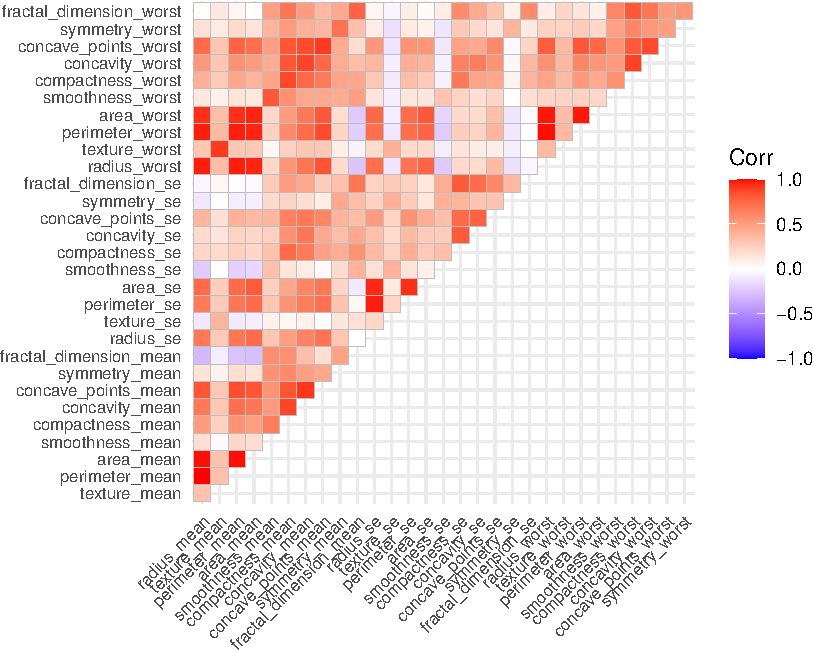
\includegraphics{Report_files/figure-latex/unnamed-chunk-2-1.pdf}

\begin{Shaded}
\begin{Highlighting}[]
\CommentTok{\#X = stand\_df \%\textgreater{}\% }
  \CommentTok{\#select(radius\_mean, texture\_mean, smoothness\_mean, compactness\_mean,}
         \CommentTok{\#symmetry\_mean, fractal\_dimension\_mean, radius\_se, texture\_se,}
         \CommentTok{\#smoothness\_se, concavity\_se, symmetry\_se)}

\CommentTok{\#corr\_new = X \%\textgreater{}\% cor()}
\CommentTok{\#corr\_new}

\CommentTok{\#ggcorrplot(corr\_new, type = "upper", lab = TRUE)}
\end{Highlighting}
\end{Shaded}

\begin{Shaded}
\begin{Highlighting}[]
\NormalTok{logdata }\OtherTok{=} \FunctionTok{cbind.data.frame}\NormalTok{(y, X)}
\NormalTok{log\_model }\OtherTok{=} \FunctionTok{glm}\NormalTok{(y }\SpecialCharTok{\textasciitilde{}}\NormalTok{ ., }\AttributeTok{family =} \FunctionTok{binomial}\NormalTok{(}\AttributeTok{link =} \StringTok{"logit"}\NormalTok{),}\AttributeTok{data =}\NormalTok{ logdata)}
\FunctionTok{summary}\NormalTok{(log\_model)}
\end{Highlighting}
\end{Shaded}

\begin{verbatim}
## 
## Call:
## glm(formula = y ~ ., family = binomial(link = "logit"), data = logdata)
## 
## Deviance Residuals: 
##    Min      1Q  Median      3Q     Max  
##  -8.49   -8.49   -8.49    8.49    8.49  
## 
## Coefficients:
##                          Estimate Std. Error z value Pr(>|z|)    
## (Intercept)                253916      23548  10.783  < 2e-16 ***
## radius_mean               8552881     948876   9.014  < 2e-16 ***
## texture_mean               842067      63252  13.313  < 2e-16 ***
## perimeter_mean           35796847     598698  59.791  < 2e-16 ***
## area_mean               -45790271    1375034 -33.301  < 2e-16 ***
## smoothness_mean          -2144100     117586 -18.234  < 2e-16 ***
## compactness_mean          -339500     169667  -2.001  0.04540 *  
## concavity_mean              83032     112278   0.740  0.45959    
## concave_points_mean       -665733     208830  -3.188  0.00143 ** 
## symmetry_mean             1109889      21306  52.093  < 2e-16 ***
## fractal_dimension_mean    -298858      15312 -19.519  < 2e-16 ***
## radius_se                 9230274     324119  28.478  < 2e-16 ***
## texture_se                3513102     110604  31.763  < 2e-16 ***
## perimeter_se              3438590      95432  36.032  < 2e-16 ***
## area_se                 -29084420     834804 -34.840  < 2e-16 ***
## smoothness_se             2249396      36747  61.213  < 2e-16 ***
## compactness_se           -3175247     102656 -30.931  < 2e-16 ***
## concavity_se              4614370     161208  28.624  < 2e-16 ***
## concave_points_se        -7773633     247582 -31.398  < 2e-16 ***
## symmetry_se               2389064      34103  70.054  < 2e-16 ***
## fractal_dimension_se      4001120     174560  22.921  < 2e-16 ***
## radius_worst            -29628795    1035752 -28.606  < 2e-16 ***
## texture_worst            -3584767     149772 -23.935  < 2e-16 ***
## perimeter_worst         -11889227     409644 -29.023  < 2e-16 ***
## area_worst               50959831    1560436  32.657  < 2e-16 ***
## smoothness_worst          -493436      75304  -6.553 5.66e-11 ***
## compactness_worst         1413874      62922  22.470  < 2e-16 ***
## concavity_worst          -6316972     317828 -19.875  < 2e-16 ***
## concave_points_worst      9408268     359616  26.162  < 2e-16 ***
## symmetry_worst           -1530342      20986 -72.923  < 2e-16 ***
## fractal_dimension_worst   -667962      96441  -6.926 4.33e-12 ***
## ---
## Signif. codes:  0 '***' 0.001 '**' 0.01 '*' 0.05 '.' 0.1 ' ' 1
## 
## (Dispersion parameter for binomial family taken to be 1)
## 
##     Null deviance:   751.44  on 568  degrees of freedom
## Residual deviance: 32006.76  on 538  degrees of freedom
## AIC: 32069
## 
## Number of Fisher Scoring iterations: 25
\end{verbatim}

\end{document}
